\documentclass[11pt]{beamer}
\usetheme{Warsaw}
\usepackage[utf8]{inputenc}
\usepackage{amsmath}
\usepackage{amsfonts}
\usepackage{amssymb}
\usepackage{graphicx}
\author{Gianluca Rossi}
\title{A primer on Bayesian Hierarchical modelling}
%\setbeamercovered{transparent} 
%\setbeamertemplate{navigation symbols}{} 
%\logo{} 
%\institute{} 
\date{January 18, 2017} 
%\subject{} 
\begin{document}

\begin{frame}
	\titlepage
\end{frame}

%%%%%%%%%%%%%%%%%%%%%%%%%%

\begin{frame}
	\tableofcontents
\end{frame}

%%%%%%%%%%%%%%%%%%%%%%%%%%

\section{A primer on Bayes' Theorem}
\subsection{The Bayes' Theorem}
\begin{frame}
	\frametitle{Some art courtesy of the University of Cambridge}
%	\framesubtitle{}
	\begin{figure}
		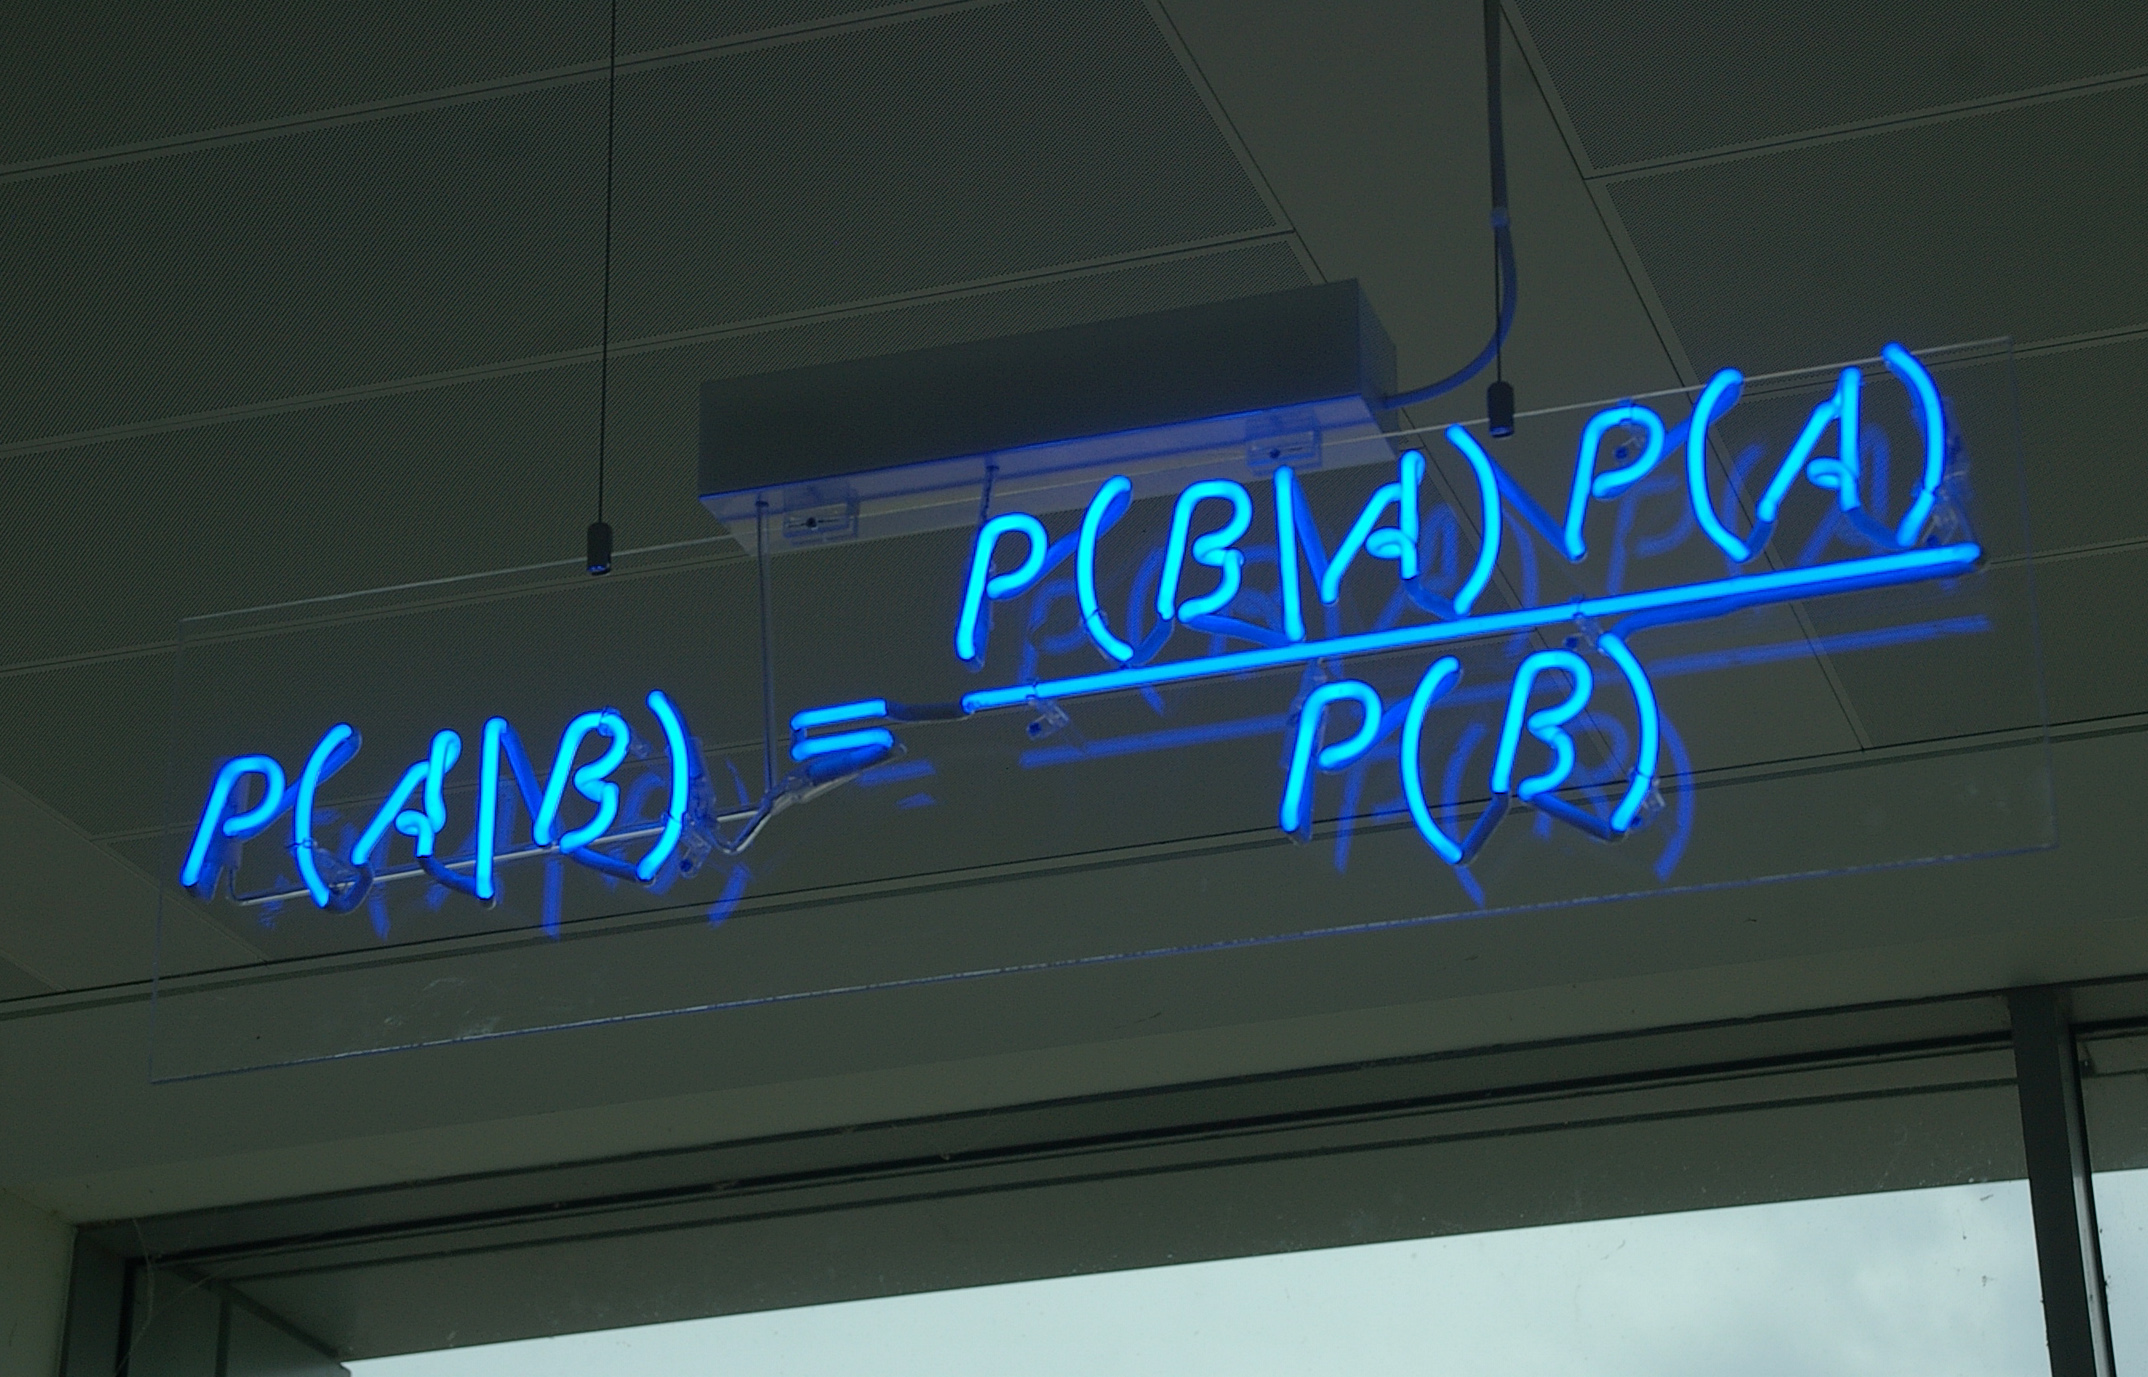
\includegraphics[scale=0.12]{./images/Bayes'_Theorem_MMB_01.jpg}
		\caption{Bayes' theorem spelt out in blue neon at the offices of Autonomy in Cambridge. (credit: \href{https://commons.wikimedia.org/wiki/User:Mattbuck}{Mattbuck, Wikipedia})}	
	\end{figure}
	
\end{frame}

\begin{frame}
	\frametitle{The exact formulation}
%	\framesubtitle{}
	Assuming we are working in a discrete space, the Bayes' Theorem can be written as:
	\begin{align}
		P(\theta | D) &= \frac{P(D | \theta) P(\theta)}{P(D)} \\
		&= \frac{P(D|\theta) P(\theta)}{\sum_{\theta^{\star}} P(D | \theta^{\star}) P(\theta^{\star})} \\
		&\propto P(D|\theta) P(\theta)
	\end{align}
	The three components of the equation are:
	\begin{itemize}
		\item $P(\theta | D)$, the posterior
		\item $P(D | \theta)$, the likelihood function
		\item $P(D)$, the normalising function
	\end{itemize}
\end{frame}

\begin{frame}
	\frametitle{The likelihood function}
%	\framesubtitle{}
	The likelihood is a function of the parameters of a statistical model given data. In other words, the likelihood describes the probability of observing the data given the parameters of the statistical model.
\end{frame}

\begin{frame}
	\frametitle{The prior distribution}
%	\framesubtitle{}
	The prior is a probabilistic formulation of our beliefs before collecting data.
	\begin{itemize}
		\item Priors can be weak, moderate or strong, depending on how concentrated the probability density is compared to the problem space
		\item In hierarchical models, priors can be implicit, thus determined by higher level's parameters
		\item It's important to investigate priors when working with complex models because these could strongly impact the final results (this is not \textit{p-hacking} or \textit{The Garden of Forking Paths})
	\end{itemize}

\end{frame}

\begin{frame}
	\frametitle{The posterior distribution}
%	\framesubtitle{}
	The posterior distribution is the updated belief after collecting new data.
	\begin{itemize}
		\item Could have the same form of the prior (\textit{conjungate} property), but this is not very interesting when dealing with complex models or using Markov Chain Monte Carlo processes (MCMC)
	\end{itemize}
\end{frame}

\subsection{Why is Bayes' Theorem useful?}
\begin{frame}
	The main reasons behind the success of Bayesian Inference are:
	\begin{itemize}
		\item It allows to take into account prior knowledge, when this is relevant
		\begin{itemize}
			\item Speed-up convergence
			\item Attribute non-zero probability to yet unobserved events (contrary to frequentist approach)
		\end{itemize}
		\item Move beyond single point estimation
		\item Estimate probability in a joint parameter space
	\end{itemize}		
\end{frame}

\subsection{Baseball example}
\begin{frame}
	Let's assume we are trying to estimate the batting performance of baseball players. We are interested on predicting the Batting Average (AVG) for 947 players, based on the 2012 MLB season statistics.
\end{frame}

\begin{frame}
	Our model is:
	\begin{align}
	z_s &\sim Binomial(N_s, \theta_s) \quad \text{ where } s \in [1, S]\\
	\theta_s &\sim Beta(\alpha, \beta) \quad \text{ where } \quad \alpha = 1 \text{ and } \beta = 1
	\end{align}
	\begin{itemize}
	\item The likelihood is a Binomial function
	\item The prior is a Beta probability distribution (Uniform)
	\item We interested in computing the posterior distribution for the Batting Average (also abbreviated AVG, $\theta$) of $S = 947$ players
	\end{itemize}
\end{frame}

\begin{frame}
	Since Binomial likelihood and Beta prior are conjungate, we can derive a solution analytically, which is very convenient to understand how everything fits within the Bayes' Theorem framework.	
\end{frame}

\begin{frame}
	Omitting the indices for clarity, we have that:
	\begin{align}
	P(\theta|z, N) &= \frac{P(z, N | \theta) P(\theta)}{P(z, N)} \\
	&= \frac{\left( \frac{N!}{z! (N-z)!} \right) \theta^z (1 - \theta)^{(N-z)} \frac{\theta^{(\alpha - 1)}(1 - \theta)^{(\beta - 1)}}{B(\alpha, \beta)}}{P(z, N)} \label{eq:beta-binomial-definition}\\
	&\propto \frac{\theta^z (1 - \theta)^{(N-z)} \frac{\theta^{(\alpha - 1)}(1 - \theta)^{(\beta - 1)}}{B(\alpha, \beta)}}{P(z, N)} \\
	&\propto \frac{\theta^{((z + \alpha) - 1)} (1 - \theta)^{((N - z + \beta) - 1)} }{B(\alpha, \beta) P(z, N)} \\
	&= \frac{\theta^{((z + \alpha) - 1)} (1 - \theta)^{((N - z + \beta) - 1)} }{B(z + \alpha, N - z + \beta)} \label{eq:posterior_beta_distribution}
	\end{align}
\end{frame}

\begin{frame}
	Notes:
	\begin{itemize}
	\item \eqref{eq:beta-binomial-definition} Plugging in the definition of Binomial and Beta distributions 
	\item For \eqref{eq:posterior_beta_distribution} to be a probability distribution, as it must be, the denominator must be the normalising factor for the corresponding Beta distribution, which is $B(z + \alpha, N - z + \beta)$
	\end{itemize}
\end{frame}

\begin{frame}
	See Stan model in \textit{baseball.ipynb} notebook
\end{frame}


\subsection{Data order sensitivity}
\begin{frame}
	A fundamental question, often underestimated, when doing Bayesian Data Analysis is: 
	\begin{block}{Data sensitivity}
	How does Bayes' Theorem weight more recent data?
	\end{block}
\end{frame}

\begin{frame}
	Starting from the Bayes' Theorem equation we can solve this problem very easily:
	\begin{align}
		P(\theta | D^{\prime}, D) &= \frac{P(D^{\prime}, D | \theta) P(\theta)}{\sum_{\theta^{\star}} P(D^{\prime}, D | \theta^{\star}) P(\theta^{\star})} \\ 
		&= \frac{P(D^{\prime} | \theta) P(D | \theta) P(\theta)}{\sum_{\theta^{\star}} P(D^{\prime} | \theta^{\star}) P(D | \theta^{\star}) P(\theta^{\star})} \\
		&= \frac{P(D | \theta) P(D^{\prime} | \theta) P(\theta)}{\sum_{\theta^{\star}} P(D | \theta^{\star}) P(D^{\prime} | \theta^{\star}) P(\theta^{\star})} \\
		&= P(\theta | D, D^{\prime})
	\end{align}
\end{frame}

\begin{frame}
	It's important to understand that in the Bayes' Theorem the posterior distribution is invariant from the ordering of the data. More recent data is weighted the same as old data. This is because Bayes' Theorem assumes a \textit{stationary scenario}. \\
	To give more weight to more recent data we need to modify the likelihood function to generate non independent data.
\end{frame}

%%%%%%%%%%%%%%%%%%%%%%%%%%

\section{Moving to Bayesian Hierarchical Modelling}
\subsection{What does hierarchical/Multilevel Modelling mean?}
\begin{frame}
	Hierarchical modelling means expressing the Bayes' Theorem as dependencies between parameters instead of an expression about the joint parameter space.
\end{frame}

\begin{frame}
	But what does this mean?
\end{frame}


\begin{frame}
	Let's improve on our previous example. We are still dealing with baseball data and want to estimate players' performance. \\
	This time however we want to have different priors based on the role of the player (\textit{pitcher}, \textit{1st base}, etc\dots). In this formulation, performance of players with a similar role will influence the final prediction for the player. \\
\end{frame}

\begin{frame}
	Differently from the previous model specification we will re-parametrise the Beta prior to use mode ($\omega$) and concentration ($\kappa$). In this way we can give hyper-priors to the parameters of the Beta prior.
	\begin{align}
	z_s &\sim Binomial(N_s, \theta_s) \quad \text{ where } s \in [1, S]\\
	\theta_s &\sim Beta(\omega_c (\kappa_c - 2) + 1, (1 - \omega_c) (\kappa_c - 2) + 1) \\
	\omega_c &\sim \dots \\
	\kappa_c &\sim \dots	
	\end{align}
\end{frame}


\begin{frame}
%	\frametitle{The Beta-Binomial model}
%	\framesubtitle{}
	Now, let's plug this into the Bayes' Theorem framework. Again, to simplify the notation we are going to omit the indices.
	
	\begin{align}
		P(\theta, \omega, \kappa | D) &= \frac{P(D | \theta, \omega, \kappa) P(\theta, \omega, \kappa)}{P(D)} \\
		&= \frac{P(D | \theta) P(\theta, \omega, \kappa)}{P(D)} \label{eq:likelihood_ind}\\
		&= \frac{P(D | \theta) P(\theta | \omega, \kappa) P(\omega, \kappa)}{P(D)} \label{eq:hierarchical_formulation}
	\end{align}
	
	We made the following steps:
	\begin{itemize}
		\item \eqref{eq:likelihood_ind} because likelihood doesn't depend on $\omega$ and $\kappa$
		\item \eqref{eq:hierarchical_formulation} because $P(\theta | \omega, \kappa) = \frac{P(\theta, \omega, \kappa)}{P(\omega, \kappa)}$, thus $P(\theta, \omega, \kappa) = P(\theta | \omega, \kappa) P(\omega, \kappa)$
	\end{itemize}
\end{frame}

\begin{frame}
%	\frametitle{}
%	\framesubtitle{}
	When dealing with a continuous problem space \eqref{eq:hierarchical_formulation} becomes:
	\begin{align}
		P(\theta_1, \dots m | D) &= \frac{P(D | \theta_1, \dots m) P(\theta_1, \dots m)}{P(D)} \\
		&= \frac{P(D | \theta_1, \dots m) P(\theta_1, \dots m)}{\sum\limits_{m} \int \mathrm{d}\theta_{m} P(D | \theta_1, \dots m) P(\theta_1, \dots m)} \\
		&= \frac{\prod P_{m}(D | \theta_{m}, m) P_{m}(\theta_{m} | m) P(m)}{\sum\limits_{m} \int \mathrm{d}\theta_{m} \prod_{m} P_{m}(D | \theta_{m}, m) P_{m}(\theta_{m} | m) P(m)}
	\end{align}		
\end{frame}


\subsection{Baseball example}
\begin{frame}
%	\frametitle{The Beta-Binomial model}
%	\framesubtitle{}
	See Stan model in \textit{baseball.ipynb} notebook
\end{frame}


\end{document}